\documentclass[11pt]{article}
\usepackage[margin=0.85in]{geometry}
\usepackage[T1]{fontenc}
\usepackage{lmodern,amsmath,amssymb,booktabs,array,graphicx,xcolor}
\usepackage[colorlinks=true,urlcolor=blue,linkcolor=blue]{hyperref}
\definecolor{ink}{RGB}{26,54,67}
\newcommand{\sinc}{\operatorname{sinc}}
\newcommand{\Tr}{\operatorname{Tr}}
\newcommand{\dd}{\mathrm{d}}
\newcommand{\Li}{\operatorname{Li}}
\setlength{\parindent}{0pt}
\setlength{\parskip}{6pt}
\hypersetup{pdftitle={Quadratic Higgs-portal interactions and a conditional measurement bridge},pdfauthor={AI-assisted research calculation prepared for the ZoraASI project}}
\begin{document}
\begin{center}
{\small\color{ink} ZORAASI RESEARCH PROGRAM \quad / \quad 11 OCTOBER 2026}\par
\vspace{8pt}
{\LARGE\bfseries Quadratic Higgs-portal interactions\par and a conditional measurement bridge}\par
\vspace{8pt}
{\large Thermal scalar scattering, mixed fields, and visibility decay}\par
\vspace{5pt}
Prepared for Christopher Michael Baird\par
AI-assisted derivation and computational audit; working note v0.1
\end{center}

\textbf{Result.} A massive free scalar has no zero-frequency noise in its
\emph{linear} field operator, but its quadratic operator has a nonzero thermal
elastic-scattering contribution. The symmetric Higgs portal supplies just such
a quadratic matter coupling. Under a declared thermal state, heavy fixed-path
probe, and weak-coupling Markov approximation, this yields a calculable
visibility-decay rate. The derivation extends to two mixed scalar mass modes.

\textbf{Scientific status.} This is a conditional application of established
Higgs-portal and open-system methods, not a claim of new fundamental physics,
experimental detection, novelty, or a completed Theory of Everything.
The existence, population, and temperature of the putative scalar bath have
not been measured. A complete laboratory model and high-energy completion
remain open. The parent goal remains completion of the full theory; this
note addresses one necessary physical interface without redefining that goal.

\section*{What this changes in the research record}
\begin{tabular}{@{}p{0.25\linewidth}p{0.69\linewidth}@{}}
\toprule
Prior unresolved issue & Result supplied here \\
\midrule
Scalar action to probe coupling & Tree-level matching gives a definite quadratic matter operator, including its sign and identical-scalar factor. \\
Massive-bath obstruction & The linear vacuum/DC obstruction survives; quadratic thermal elastic scattering opens a different channel. \\
Arbitrary visibility coefficient & A conditional rate follows from masses, portal matrix, bath temperature, and path separation. No exponential field gate is assumed. \\
Two-scalar mixing & An ordered-pair spectral sum includes both diagonal scattering and mixed-species conversion. \\
Common-mode null & Equal means cancel phase, but do not generally cancel fluctuating path information. \\
Distance law & Quadratic growth applies at small separation; single-scalar rates saturate at large separation. \\
\bottomrule
\end{tabular}

\textbf{Units and notation.} Throughout, $\hbar=c=k_B=1$;
$T$ is bath temperature, $\tau$ is interrogation time, $r$ is path separation,
$m$ is a scalar mass, and $m_h$ is the Higgs mass. Temperature is not
interrogation time. To convert the rate to inverse seconds divide its energy
value by $\hbar$; physical distance enters as $r/(\hbar c)$ in inverse-energy units.
No numerical laboratory parameters are assigned.

\newpage
\section{From the stated portal to matter}
Use metric signature $(+---)$ and the potential convention of the September
two-singlet audit in the supplied corpus [1]:
\begin{equation}
 V\supset \tfrac12\kappa\phi^2H^\dagger H,\qquad
 H=\begin{pmatrix}0\\(v+h)/\sqrt2\end{pmatrix}.
\end{equation}
For an elementary fermion, the terms linear in the physical unmixed Higgs are
\begin{equation}
 \mathcal L\supset-\tfrac12h(\Box+m_h^2)h-hJ_h,\qquad
 J_h=\tfrac12\kappa v\phi^2+\frac{m_f}{v}\bar f f.
\end{equation}
Completing the square, at momenta small compared with $m_h$,
\begin{equation}
 \Delta\mathcal L=\tfrac12J_h(\Box+m_h^2)^{-1}J_h
 \supset c_f\phi^2\bar f f,\qquad c_f=\frac{\kappa m_f}{2m_h^2}.
 \label{eq:match}
\end{equation}
For a nucleon define $f_N$ by
$\mathcal L_{hNN}=-(f_Nm_N/v)h\bar NN$. Then
$c_N=\kappa f_Nm_N/(2m_h^2)$. In the nonrelativistic limit,
\begin{equation}
 H_{\rm int}=-c_a\int\dd^3x\,n_a(x)[\phi^2(x)]_R.
 \label{eq:matter}
\end{equation}
The positive Lagrangian coefficient becomes a negative potential-energy
coefficient. Rates below depend on $c_a^2$, so this sign does not affect them.
The $\phi\phi\bar ff$ vertex is $i\,2c_f$, not $ic_f$.

\textbf{Scattering normalization.} For scalar--nucleon scattering at low
velocity, Eq.~\eqref{eq:match} gives
\begin{equation}
 \sigma_{\phi N}=\frac{\kappa^2 f_N^2m_N^4}
 {4\pi m_h^4(m+m_N)^2}
 \ \longrightarrow\ \frac{c_N^2}{\pi}\quad(m\ll m_N).
 \label{eq:sigma}
\end{equation}
This agrees with Eq.~8 of Athron et al. [2] in the same portal normalization.
For a composite atom or extended object, its response and form factor must
be derived; a nucleon coefficient must not be silently promoted to an optical
or macroscopic detector coefficient.

\subsection*{Two mixed scalars}
For a real interaction-basis vector $\varphi$ and real symmetric portal
matrix $K=K^T$, write $V\supset\tfrac12\varphi^TK\varphi H^\dagger H$.
An orthogonal rotation $\varphi=Rs$ diagonalizes the physical singlet
mass matrix. With an unmixed Higgs and exact symmetric vacuum, the probe sees
\begin{equation}
 B=s^TCs,\qquad C=\frac{f_am_a}{2m_h^2}R^TKR,
 \qquad H_{\rm int}=-P_LB_L-P_RB_R.
 \label{eq:matrix}
\end{equation}
Here $f_a=1$ for an elementary fermion in the matching approximation;
for nucleons it is defined above. All scalar masses must be positive for
the massive equilibrium branch used here. Higgs--singlet mixing, appreciable
self-interactions, and additional mediators require new matching.
Off-diagonal $C$ preserves simultaneous inversion $s\mapsto-s$;
separate sign flips of individual mass modes need not be symmetries.

\textbf{Source constraint.} The matter term yields
$(\Box+m^2)\phi=2c_an_a\phi+\cdots$, or its matrix counterpart
$(\Box I+M^2)s=2n_aCs+\cdots$. It changes the local mass matrix;
it does not provide an additive source independent of the field.
Classical zero field remains a solution. A thermal population is additional
state information, not a consequence of this matching.

\newpage
\section{The thermal quadratic spectrum}
For one free real scalar in homogeneous equilibrium at zero chemical
potential, define
\begin{equation}
 \omega_k=\sqrt{k^2+m^2},\quad n(\epsilon)=\frac1{e^{\epsilon/T}-1},\quad
 \dd\mu_k=\frac{\dd^3k}{(2\pi)^3\,2\omega_k}.
\end{equation}
Let $O=:\!\phi^2\!:$ and center it by subtracting its thermal mean.
Vacuum normal ordering is the convention at this free-field order.
Wick contraction gives, away from coincident-distribution ambiguities,
\begin{align}
 G^>(t,\mathbf r)&=\int\dd\mu_k\big[(1+n_k)e^{-i\omega_kt+i\mathbf k\cdot\mathbf r}
                         +n_ke^{i\omega_kt-i\mathbf k\cdot\mathbf r}\big],\\
 C_O^>(t,\mathbf r)&=\langle\delta O(t,\mathbf r)\delta O(0,0)\rangle
                   =2[G^>(t,\mathbf r)]^2.\label{eq:wick}
\end{align}
Define a two-sided spectrum by $S_O(\Omega,r)=\int\dd t\,
e^{i\Omega t}C_O^>(t,\mathbf r)$. At zero frequency the pair terms cannot
contribute: $\omega_k+\omega_p\geq2m$. Elastic thermal terms do contribute:
\begin{equation}
 S_O(0,r)=8\pi\int\dd\mu_k\dd\mu_p\,n_k(1+n_p)
 \delta(\omega_k-\omega_p)e^{i(\mathbf k-\mathbf p)\cdot\mathbf r}.
\end{equation}
The angular shell integral is
\begin{equation}
 \int\dd\mu_k\,\delta(\epsilon-\omega_k)e^{i\mathbf k\cdot\mathbf r}
 =\frac{\sqrt{\epsilon^2-m^2}}{4\pi^2}
   \sinc\!\left(r\sqrt{\epsilon^2-m^2}\right).
\end{equation}
Consequently,
\begin{equation}
 \boxed{S_O(0,r)=\frac1{2\pi^3}\int_m^\infty\dd\epsilon\,
 (\epsilon^2-m^2)n(\epsilon)[1+n(\epsilon)]
 \sinc^2\!\left(r\sqrt{\epsilon^2-m^2}\right).}\label{eq:spectrum}
\end{equation}
Here $\sinc z=\sin z/z$ with $\sinc0=1$.
The zero-frequency symmetrized spectrum equals this expression; no
additional factor of two is needed.

\subsection*{Independent momentum-transfer representation}
Fourier transform Eq.~\eqref{eq:spectrum} in space. Equal bath energies
fix the longitudinal incoming momentum to $Q/2$, giving, for $Q>0$,
\begin{equation}
 \widetilde S_O(0,Q)=\frac{T}{2\pi Q}
 n\!\left(\sqrt{m^2+Q^2/4}\right).\label{eq:qspec}
\end{equation}
This is nonnegative, so all finite spatial covariance matrices are
positive semidefinite. Its integrable $1/Q$ behavior for $m>0$ does not
justify substituting the exactly global, conserved $Q=0$ coupling.
Numerical Fourier inversion supplies an independent normalization check.

At coincident positions the finite thermal coefficient is
\begin{equation}
 S_O(0,0)=\frac{-mT^2\ln(1-e^{-m/T})+T^3\Li_2(e^{-m/T})}{\pi^3}.
 \label{eq:local}
\end{equation}
It follows by using $n(1+n)=-T\partial_\epsilon n$ and integrating
by parts. In particular $[S_O]={\rm energy}^3$.

\newpage
\section{Visibility decay and the mixed-field extension}
For a heavy probe with stationary paths, the local coupling is
$H_{\rm int}=-c_a(P_LO_L+P_RO_R)$. Assume weak coupling, an effectively
infinite stationary bath, and a controlled Markov approximation.
The leading generator has the positive coefficient matrix
$c_a^2S_O(0,|\mathbf x_i-\mathbf x_j|)$:
\begin{equation}
 \mathcal L\rho=c_a^2\sum_{i,j=L,R}S_{ij}
 \left(P_j\rho P_i-\tfrac12\{P_iP_j,\rho\}\right).
\end{equation}
Its off-diagonal matrix element decays as
\begin{equation}
 \gamma(r)=c_a^2[S_O(0,0)-S_O(0,r)],\qquad
 \frac{V(\tau)}{V_{\rm reference}(\tau)}\simeq e^{-\gamma(r)\tau}.
 \label{eq:rate}
\end{equation}
The reference must remove this scalar channel while treating all ordinary
instrument effects consistently. It is a theoretical reference here.
The path populations remain unchanged under this pure-dephasing generator;
the final recombination fringe follows the ordinary Born rule.

\textbf{Independent collision check.} In the heavy-target Born limit,
$\sigma=c_a^2/\pi$ from Eq.~\eqref{eq:sigma}. Multiplying the thermal
number density by speed $k/\omega_k$, Bose final-state enhancement,
and isotropic path distinguishability gives
\begin{equation}
 \gamma(r)=\frac{c_a^2}{2\pi^3}\int_0^\infty\dd k\,
 \frac{k^3}{\omega_k}n_k(1+n_k)[1-\sinc^2(kr)].
\end{equation}
Changing variable to $\epsilon=\omega_k$ reproduces
Eq.~\eqref{eq:rate}. This connects the coefficient to conventional
thermal collisional decoherence [3], rather than a modified Born rule.

\subsection*{Full quadratic coupling of two independent mass modes}
For Eq.~\eqref{eq:matrix}, with the modes at a common temperature,
$\langle\delta B(x)\delta B(0)\rangle=2\sum_{ij}C_{ij}^2G_i^>(x)G_j^>(x)$.
Set $k_i(\epsilon)=\sqrt{\epsilon^2-m_i^2}$ on its allowed shell.
The same calculation gives
\begin{equation}
\boxed{\begin{aligned}
\gamma_{\rm mixed}(r)&=\frac1{2\pi^3}\sum_{i,j}C_{ij}^2
 \int_{\max(m_i,m_j)}^\infty\dd\epsilon\,
 k_i k_j n(\epsilon)[1+n(\epsilon)]\\[-2pt]
&\hspace{21mm}\times[1-\sinc(k_ir)\sinc(k_jr)].
\end{aligned}}\label{eq:mixed}
\end{equation}
Both $i\ne j$ orderings are included. A mixed coupling can convert one
species into the other at the same energy; this requires the threshold
$\epsilon\ge\max(m_i,m_j)$. The fixed heavy probe absorbs momentum
with negligible recoil energy. A finite-mass probe needs recoil kinematics.

Every integrand in Eq.~\eqref{eq:mixed} is nonnegative. If all masses
coincide, the answer is proportional to $\Tr(C^2)$ and is invariant under
orthogonal changes of the degenerate basis. For unequal masses, the
cross-spectrum can have negative spatial values; the one-field bound
$\gamma\le S_B(0,0)$ must be replaced by $\gamma\le2S_B(0,0)$.

\newpage
\section{Limits that can falsify an implementation}
For one scalar, Eqs.~\eqref{eq:spectrum}--\eqref{eq:rate} imply
\begin{align}
 0&\le\gamma(r)\le c_a^2S_O(0,0),&\gamma(0)&=0,\\
 \gamma(r)&=\frac{c_a^2r^2}{6\pi^3}\int_m^\infty\dd\epsilon\,
 (\epsilon^2-m^2)^2n(1+n)+O(r^4),\\
 \gamma(\infty)&=c_a^2S_O(0,0),&
 S_O(0,r)&\sim\frac{Tn(m)}{4\pi^3r^2}\quad(r\to\infty).
\end{align}
The small-distance expansion requires $kr\ll1$ over the populated modes.
It does not apply when the arms are already decorrelated.

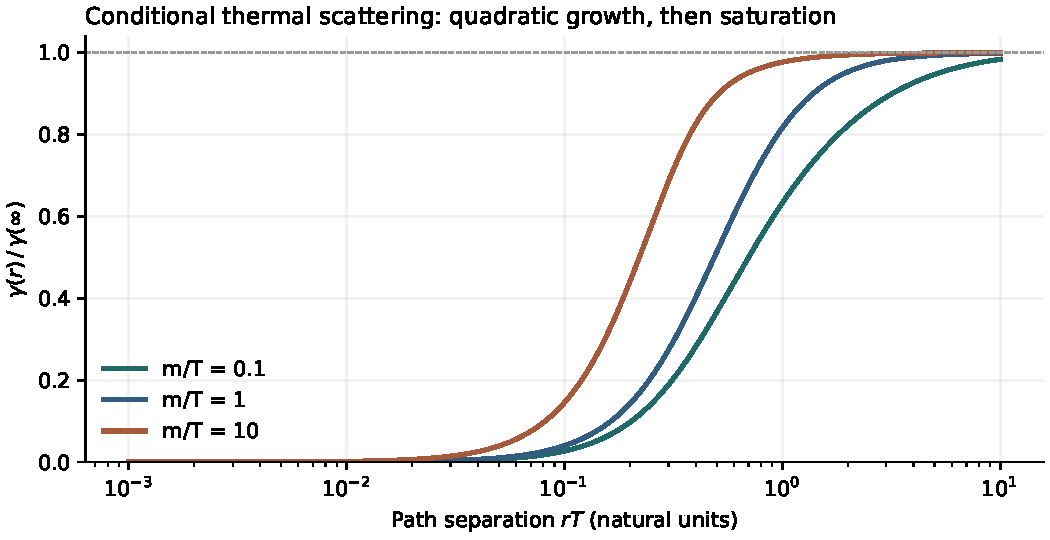
\includegraphics[width=\linewidth]{rate_shape.pdf}

\textbf{Plot.} Deterministic evaluation of the conditional formula, normalized
separately by each curve's saturation rate. The curves are not observations;
normalization hides the strong mass/temperature dependence of their amplitudes.

For $T\ll m$, the leading local spectrum is
\begin{equation}
 S_O(0,0)\simeq\frac{(mT^2+T^3)e^{-m/T}}{\pi^3}.
\end{equation}
The suppression is $e^{-m/T}$, since one existing thermal particle scatters.
For $r\sqrt{mT}\ll1$ as well,
$\gamma(r)\sim4c_a^2m^2T^3r^2e^{-m/T}/(3\pi^3)$.
As $m/T\to0$, the local coefficient approaches $T^3/(6\pi)$;
this limiting coefficient alone does not establish every massless Markov assumption.

\textbf{Vacuum boundary.} At $T=0$ the zero-frequency rate vanishes for
$m>0$. Vacuum pair production starts at $2m$. This statement concerns the
long-time leading rate and does not exclude switching transients, dressing,
or finite-time entanglement with the vacuum.

\textbf{Equal means are not a null.} A homogeneous bath has
$\langle O_L\rangle=\langle O_R\rangle$ and therefore no mean relative
phase, but its difference noise is nonzero for $r>0$. At $m/T=1,rT=1$,
the calculated rate is about $0.8162$ of its large-separation value.
Exact cancellation requires identical coupled fluctuations, not just equal
classical background values.

\newpage
\section{Using the same portal in collider and visibility calculations}
An additional consistency relation follows without choosing a portal
strength. For one real scalar with $2m<m_h$, the tree-level Higgs partial
width in this convention [2] is
\begin{equation}
 \Gamma_{h\to\phi\phi}=\frac{\kappa^2v^2}{32\pi m_h}\beta,
 \qquad\beta=\sqrt{1-4m^2/m_h^2}>0.
\end{equation}
Eliminating $\kappa^2$ between this expression and Eq.~\eqref{eq:match}
gives a conditional relation to the heavy-nucleon visibility rate:
\begin{equation}
 \boxed{\gamma_N(r)=\frac{8\pi f_N^2m_N^2}{v^2m_h^3\beta}
 \Gamma_{h\to\phi\phi}\,[S_O(0,0)-S_O(0,r)].}\label{eq:collider}
\end{equation}
This relation uses the same portal parameter on both sides. It avoids
treating the interferometric rate as a freely adjustable coefficient once
the scalar state and physical matching are specified.

If both daughters are invisible in the collider detector, a valid upper
limit on the total invisible width also bounds this partial width. It can
then be inserted into Eq.~\eqref{eq:collider}, conditionally on the scalar
mass and bath spectrum. No current collider limit is inserted here and no
new experimental exclusion is claimed. A branching-fraction limit also
requires a consistent total-width model before conversion to a partial-width
bound. At threshold $\beta=0$ the division is invalid; near threshold the
inferred bound becomes weak.

\subsection*{Degenerate mixed modes}
When all included scalar mass modes have the same mass and thermal
propagator, the inclusive sector width is
\begin{equation}
 \Gamma_{h\to ss}=\frac{v^2\beta}{32\pi m_h}\Tr(K^2).
\end{equation}
The diagonal channels carry the identical-particle factor; each distinct
pair contributes twice a diagonal channel with the same portal entry.
Since $\gamma=\Tr(C^2)\Delta S_O$, the same relation
\eqref{eq:collider} holds with this inclusive sector width. Applying an
invisible-width bound requires every included daughter mode to be
invisible in the detector. Mass degeneracy
alone is insufficient when populations, interactions, or thermal mass
corrections distinguish the modes. Nondegenerate modes require their own
phase-space factors and Eq.~\eqref{eq:mixed}.

\subsection*{Optional naturalness restriction, explicitly conditional}
If one further imposes $m^2=m_0^2+\kappa v^2/2$ with
$m_0^2\ge0$ and $\kappa\ge0$, then
\begin{equation}
 \kappa\le\frac{2m^2}{v^2},\qquad
 \gamma_N(r)\le\frac{f_N^2m_N^2m^4}{v^4m_h^4}\,
 [S_O(0,0)-S_O(0,r)].
\end{equation}
This is a no-cancellation prior for the stated mass decomposition, not a
bound implied by symmetry or a proof of loop-level naturalness. A protected
or tuned construction may not obey it. Running couplings, thresholds,
Higgs mixing, and quantum corrections require consistent matching before
the tree-level relations can support a precision comparison.

\textbf{Remaining empirical obstruction.} A collider measurement constrains
interactions, not the local occupation of an unobserved scalar bath. Without
independent state information, Eq.~\eqref{eq:collider} cannot assign a
numerical laboratory visibility signal.

\newpage
\section{Validity, unresolved inputs, and experimental meaning}
The underlying scalar state is Gaussian; the quadratic operator is not.
Equation~\eqref{eq:wick} fixes its two-point function but does not eliminate
higher connected cumulants. Exponential visibility is a leading
weak-coupling Markov prediction, not an exact finite-coupling solution.
Weak-coupling limits require technical hypotheses [4]; they are not proved
for every unbounded composite-field model by writing a Lindblad equation.

\textbf{Regulation.} Normal ordering removes the vacuum mean, not every
coincident-point divergence. Use a smooth regulator on each field mode,
for example $F_\Lambda(k)=e^{-k^2/(2\Lambda^2)}$, before making the
full dynamical calculation. The one-scalar thermal integrand receives
$F_\Lambda(k)^4$ and has a finite limit as $\Lambda\to\infty$.
This is a statement about the displayed thermal coefficient; it does not
renormalize all Lamb shifts or higher orders. Related scalar open-system
calculations exhibit finite-time renormalization issues [5], and quadratic
detectors have additional ultraviolet subtleties [6]. A physical EFT cutoff
must remain below its breakdown scale; taking the convergent thermal
integral to infinity is justified only when its relevant modes lie well below it.

\textbf{Scale and state requirements.} Higgs matching requires relevant
momentum transfers small compared with $m_h$. Probe recoil, appreciable
scalar interactions, spatially varying populations, field-dependent
detector response, and bath backreaction require further work. A bath at
temperature $T$ is a stipulated state, not evidence of thermalization or a
cosmological abundance. Take the continuum bath limit before the long-time
limit; a finite free box has recurrences. The coupling must remain weak
on the regulated bath's correlation timescale.

\textbf{What an experiment could constrain.} With a measured or independently
justified scalar state and an apparatus transfer model, visibility data can
constrain Eq.~\eqref{eq:rate} or Eq.~\eqref{eq:mixed}. Without such state
information, an absent signal cannot bound the portal coupling independently
of scalar abundance: the bath can simply be unpopulated. Even a nonzero
decoherence rate does not uniquely identify a scalar mechanism.
The massless limiting amplitude $c_a^2T^3/(6\pi)$ makes an amplitude-only
coupling/temperature degeneracy explicit.

\textbf{Required measurement model.} The next empirical step needs a named
matter-wave probe, physical path profiles and duration, bath-state bounds,
the associated coupling/form factor, a visibility likelihood including
ordinary scattering and technical noise, and an independently calibrated
reference. This note does not supply a photon Mach--Zehnder response by
substituting nucleon parameters. No laboratory data were collected and no
discovery is inferred.

\textbf{Relation to earlier mechanisms.} This is an equilibrium thermal
quadratic-portal branch. It neither derives nor assumes
$\gamma_k(E)=\gamma_{k0}e^{\eta_k E}$, a hidden $S^2E$ source, or the
interpretive identification of fields with consciousness or ethics.
Its role is to test a physical interaction already present in the corpus,
not to declare all proposed mechanisms equivalent.

\newpage
\section{Verification record and corrections}
\texttt{check\_quadratic\_bridge.py} evaluates the derived expressions and
writes \texttt{checks.json}. The final script hash, versions, and numerical
results are recorded there. All calculations are theoretical; no laboratory
or simulated detection data are used.

\begin{tabular}{@{}p{0.49\linewidth}p{0.45\linewidth}@{}}
\toprule
Check & Scope \\
\midrule
Energy integral vs dilogarithm & Local thermal coefficient and factors of $\pi$.\\
Spatial Fourier inversion & Independent momentum-transfer representation.\\
Scattering flux vs noise rate & Portal vertex and visibility-rate normalization.\\
Finer grid and longer integration range & Numerical resolution and thermal tail.\\
Small separation and low/high temperature & Limiting formulas and domain checks.\\
Eight-position covariance matrix & Numerical positivity check in a nontrivial geometry.\\
Regulated thermal rates & Convergence of this coefficient only.\\
Mixed masses and degenerate rotation & Thresholds, off-diagonal counting, basis invariance.\\
\bottomrule
\end{tabular}

The first coarse energy grid missed rapid oscillations in one corner of the
test range. Increasing its resolution removed a relative discrepancy of
about $6.8\times10^{-6}$. The comparison is retained as a reason for the
resolution check, rather than treating the first passing-looking values as final.
The numerical tests support the stated formulas; they are not a proof of
their application to an actual device.

\subsection*{Two corrections to preserve alongside the historical note}
The corrected 11 September reservoir note [7] still introduces a
$\lambda(E_L-E_R)P_L\otimes B$ gate while describing a two-monitor repair.
This is an additional differential-controller model; it does not follow
from two local portal interactions. Physical access to both backgrounds
needs causal transport or an explicitly justified quasi-static approximation.
Equal average backgrounds do not establish its proposed null for the
local quadratic interaction derived here.

That note also associates the spatial quadratic law with
$\ell_c\ll\Delta x$. In a smooth correlated bath, the Taylor regime is
$\Delta x\ll\ell_c$ for the relevant modes. Large separation yields
saturation in the one-scalar model. These findings are recorded as an
addendum; the historical source has not been silently rewritten.

\subsection*{Current claim boundary}
Portal matching, the free thermal spectral integrals, and the leading
conditional visibility law have explicit derivations and computational
cross-checks. Finite-time renormalized dynamics, measured bath inputs,
device calibration, global parameter compatibility, quantum gravity,
high-energy completion, and independent experimental replication remain
open. Internal AI cross-checks are not external scientific verification.

\newpage
\section{Public experimental data located for the next test}
The user reported no apparatus and asked that existing data be found.
The following public data were located on 11 October 2026. Their availability
does not establish the proposed scalar interaction. The derivation and
numerical checks above do not fit these measurements.

\textbf{Lattice atom interferometry.}
Panda et al., \emph{Coherence limits in lattice atom interferometry at the
one-minute scale}, Nature Physics (2024),
\href{https://doi.org/10.1038/s41567-024-02518-9}{doi:10.1038/s41567-024-02518-9}.
The paper links an open figure-data deposit. Both its original version
and the newer \href{https://zenodo.org/records/15227841}{Zenodo record 15227841}
were retrieved; all five files in each version passed their published MD5
checksums. The newer files include contrast versus hold time and measured
fringes. These are published figure data, not a complete record of every
experimental event or systematic uncertainty. The old and new files are
not interchangeable: both figure numbering and values change.

\textbf{A data-quality issue to resolve before fitting.}
The newer Figure 3a file has nine rows. Its last two rows have identical
contrast and uncertainty, at very slightly different times near 70.071 s.
They may represent the same measurement. They must not silently be counted
as two independent observations. The record does not supply a full
covariance matrix or a scalar-free visibility reference. The paper identifies
ordinary apparatus dephasing, so observed contrast loss cannot be assigned
to a new field by subtraction without an apparatus model.

\textbf{Sodium-cluster matter-wave interferometry.}
Pedalino et al., \emph{Probing quantum mechanics with nanoparticle matter-wave
interferometry}, Nature 649, 866--870 (2026),
\href{https://doi.org/10.1038/s41586-025-09917-9}{doi:10.1038/s41586-025-09917-9}.
The linked \href{https://zenodo.org/records/17502163}{Zenodo record 17502163}
contains measurement scans, mass spectra, a settings workbook, and analysis
code. Its 88,626-byte archive was downloaded and its published MD5 checksum
verified. This is a candidate for an apparatus-specific visibility analysis.
The archive's code was inspected as source and was not executed. The
published agreement with ordinary quantum interference does not establish
a new scalar bath. Both Zenodo datasets carry CC BY 4.0 licenses.

\textbf{Collider complement.}
The \href{https://atlas.web.cern.ch/Atlas/GROUPS/PHYSICS/PAPERS/HIGG-2021-05/index.php}
{ATLAS HIGG-2021-05 public result} supplies invisible-Higgs branching-fraction
constraints and likelihood-scan plots. These can constrain the portal under
the experimental production and decay assumptions. A plotted likelihood
is not automatically a downloaded numerical likelihood, and an exclusion
limit is not a detection. A numerical reinterpretation is deferred until its
input and width assumptions have been checked.

\textbf{Local evidence and next step.}
A local magnetometer CSV matches the recovered pilot's recorded hash,
but the accompanying account describes uncontrolled phone orientation and
motion. Existing project interferometry fixtures are labeled synthetic.
Neither is a measured test of Eq.~\eqref{eq:rate}. The next defensible step
is to reproduce a public interferometer's baseline analysis, resolve data
provenance issues, and derive its finite-path and composite-probe response
before adding the scalar channel. Bath-state information remains necessary.
The companion data catalog records locations, checksums, and these limits.

\newpage
\section*{Sources and reproducibility}
\begin{enumerate}
\item C. M. Baird / ZoraASI research collection, supplied four-part edition.
Volume 4, physical PDF pp.\ 1706--1711: \emph{A Two-Singlet Effective Theory
and Its Experimental Interfaces}, 21 September 2026, v0.2.
Volume 1, pp.\ 248--255: \emph{A Conditional Mathematical Scaffold}.
These are source proposals and audits, not independent validation.
\item P. Athron et al., \emph{Status of the scalar singlet dark matter model},
Eur. Phys. J. C 77, 568 (2017), especially Eqs.\ 1 and 8.
\href{https://doi.org/10.1140/epjc/s10052-017-5113-1}{doi:10.1140/epjc/s10052-017-5113-1}.
Used for the conventional portal normalization and scattering cross-check;
its historical parameter constraints are not imported as current bounds.
\item K. Hornberger and J. E. Sipe, \emph{Collisional decoherence reexamined},
Phys. Rev. A 68, 012105 (2003).
\href{https://arxiv.org/abs/quant-ph/0303094}{arXiv:quant-ph/0303094}.
Context for scattering-induced path decoherence and normalization discipline.
\item E. B. Davies, \emph{Markovian master equations}, Commun. Math. Phys.
39, 91--110 (1974).
\href{https://doi.org/10.1007/BF01608389}{Publisher record}.
Context for conditional weak-coupling limits; not a claim that every hypothesis
has been established for the full interacting scalar apparatus.
\item C. Burrage, C. K\"ading, P. Millington and J. Min\'a\v r,
\emph{Open quantum dynamics induced by light scalar fields}.
\href{https://arxiv.org/abs/1812.08760}{arXiv:1812.08760}.
Related Higgs-portal open dynamics and finite-time renormalization.
\item A. Sachs, R. B. Mann and E. Mart\'in-Mart\'inez,
\emph{Entanglement harvesting and divergences in quadratic Unruh--DeWitt
detectors pairs}, Phys. Rev. D 96, 085012 (2017).
\href{https://arxiv.org/abs/1704.08263}{arXiv:1704.08263}.
Different detector setting illustrating why composite-coupling UV control
cannot be inferred from normal ordering alone.
\item \emph{Reservoir derivation and fail-closed interferometric protocol for
the MQGT--SCF rate-modulated GKSL sector}, corrected edition,
11 September 2026. Local source in \path{work/gate1-public/}:\\
{\small\path{Reservoir_Protocol_Note_2026-09-11_CORRECTED.tex}},
especially lines 305--359 and 477--481 in the inspected snapshot.
\end{enumerate}

\textbf{Reproduction.} In an environment with Python, NumPy, mpmath and
Matplotlib, run \texttt{python check\_quadratic\_bridge.py --plot} in the
research directory. Build this note with two passes of
\texttt{pdflatex quadratic\_portal\_measurement\_bridge.tex}.
The separate JSON manifest records source and output hashes.

\textbf{Attribution and review.} Prepared by ChatGPT/Codex in the ZoraASI
project at the user's request. Separate internal agents checked the portal
matching and the thermal spectral derivation. They are computational
cross-checks, not unaffiliated reviewers or experimental witnesses.
No claim of approval, coauthorship, or endorsement by cited authors is made.
Original synced sources and attached PDFs were kept unchanged.
\end{document}
